\documentclass{article}

% content/resources/templates/preamble.tex
\usepackage[margin=0.6in]{geometry}
\author{Milav Dabgar}
\usepackage{amsmath,amssymb,amsthm}
\usepackage{booktabs}
\usepackage{multirow}
\usepackage{xcolor}
\usepackage{tcolorbox}
\tcbuselibrary{breakable,skins}
\usepackage[colorlinks=true,linkcolor=blue]{hyperref}
\usepackage{titlesec}
\usepackage{enumitem}
\usepackage{tikz}
\usepackage{pgfplots}
\usepackage{circuitikz}
\usepackage[version=4]{mhchem}
\usepackage{longtable}
\usepackage{array}
\usepackage{float}
\usepackage{caption}
\usepackage{listings}

\lstset{
  basicstyle=\small\ttfamily,
  breaklines=true,
  breakatwhitespace=false,
  postbreak=\mbox{\textcolor{red}{$\hookrightarrow$}\space},
  float=false,
  numbers=left,
  numberstyle=\tiny\color{gray},
  numbersep=10pt,
  xleftmargin=2em,
  keywordstyle=\color{blue},
  commentstyle=\color{green!60!black},
  stringstyle=\color{purple},
  backgroundcolor=\color{gray!5},
  showstringspaces=false,
  tabsize=2,
  captionpos=b,
  keepspaces=true,
  columns=flexible
}

\pgfplotsset{compat=1.18}
\usetikzlibrary{shapes,arrows,positioning,calc,patterns,decorations.pathmorphing,decorations.markings,arrows.meta}

% Color scheme
\definecolor{headcolor}{RGB}{0,102,204}
\definecolor{keycolor}{RGB}{220,20,60}
\definecolor{solutioncolor}{RGB}{34,139,34}
\definecolor{mnemoniccolor}{RGB}{148,0,211}
\definecolor{codecolor}{RGB}{0,0,100}

% Spacing
\setlength{\parskip}{3pt}
\setlist[itemize]{nosep}
\setlist[enumerate]{nosep}

% Title formatting
\titleformat{\section}{\Large\bfseries\color{headcolor}}{\thesection}{1em}{}
\titleformat{\subsection}{\large\bfseries\color{headcolor}}{\thesubsection}{1em}{}

% Pandoc tightlist compatibility
\providecommand{\tightlist}{%
  \setlength{\itemsep}{0pt}\setlength{\parskip}{0pt}}

% Pandoc longtable compatibility
\newcounter{none}
\def\thenone{}


% content/resources/templates/english-boxes.tex

% Custom environments
\newtcolorbox{solutionbox}{
 breakable,
 enhanced,
 colback=solutioncolor!5!white,
 colframe=solutioncolor!75!black,
 fonttitle=\bfseries,
 title=Solution
}

\newtcolorbox{solutionboxnobreak}{
 colback=solutioncolor!5!white,
 colframe=solutioncolor!75!black,
 fonttitle=\bfseries,
 title=Solution
}

\newtcolorbox{keyformula}{
 breakable,
 enhanced,
 colback=keycolor!5!white,
 colframe=keycolor!75!black,
 fonttitle=\bfseries,
 title=Key Formula
}

\newtcolorbox{mnemonicboxenv}{
 breakable,
 enhanced,
 colback=mnemoniccolor!5!white,
 colframe=mnemoniccolor!75!black,
 fonttitle=\bfseries,
 title=Mnemonic
}

\newcommand{\mnemonicbox}[1]{%
  \begin{mnemonicboxenv}
    #1
  \end{mnemonicboxenv}
}


% Custom commands for GTU solutions
% This file defines semantic commands for consistent formatting

% Question command with automatic formatting
\newcommand{\question}[2]{%
  \section*{Question #1}%
  \textbf{#2}%
}

% OR question variant
\newcommand{\questionor}[2]{%
  \section*{Question #1 OR}%
  \textbf{#2}%
}

% Proper table environment with caption
\newenvironment{answertable}[1]{%
  \begin{table}[htbp]
  \centering
  \caption{#1}
}{%
  \end{table}
}

% Proper figure environment for diagrams
\newenvironment{answerdiagram}[1]{%
  \begin{figure}[htbp]
  \centering
  \caption{#1}
}{%
  \end{figure}
}

% Semantic markup for key terms
\newcommand{\keyword}[1]{\textbf{#1}}
\newcommand{\code}[1]{\texttt{#1}}
\newcommand{\classname}[1]{\texttt{#1}}
\newcommand{\methodname}[1]{\texttt{#1}}

% Proper quotation marks
\newcommand{\mnemonic}[1]{``#1''}


\title{VLSI Technology (4353206) - Winter 2024 Solution}
\date{November 29, 2024}

\begin{document}
\maketitle

\questionmarks{1(a)}{3}{Draw all symbols for enhancement and depletion type MOSFET.}

\begin{solutionbox}
\textbf{MOSFET Symbols:}

\begin{center}
\begin{tabulary}{\linewidth}{C C}
\textbf{Enhancement Type} & \textbf{Depletion Type} \\
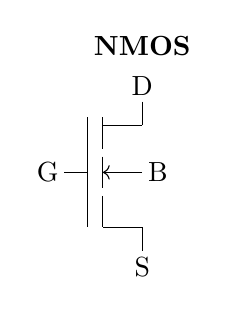
\begin{tikzpicture}[scale=1]
    % NMOS Enhancement
    \node at (0,2) {\textbf{NMOS}};
    \node at (0,1.5) {D};
    \draw (0,1.3) -- (0,1);
    \draw (0,1) -- (-0.5,1); % Drain line
    
    % Broken channel
    \draw (-0.5,1.1) -- (-0.5,0.7);
    \draw (-0.5,0.6) -- (-0.5,0.2);
    \draw (-0.5,0.1) -- (-0.5,-0.3);
    
    % Source
    \draw (0,-0.3) -- (-0.5,-0.3);
    \draw (0,-0.3) -- (0,-0.6);
    \node at (0,-0.8) {S};
    
    % Gate
    \draw (-0.7,1.1) -- (-0.7,-0.3);
    \draw (-0.7,0.4) -- (-1,0.4);
    \node at (-1.2,0.4) {G};
    
    % Body/Arrow
    \draw (-0.5,0.4) -- (0,0.4);
    \node at (0.2,0.4) {B};
    \draw[->] (0,0.4) -- (-0.5,0.4); % Arrow IN for NMOS
\end{tikzpicture}
&
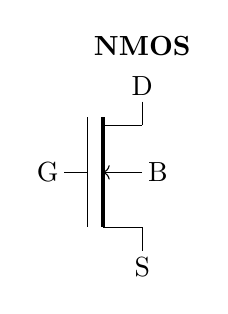
\begin{tikzpicture}[scale=1]
    % NMOS Depletion
    \node at (0,2) {\textbf{NMOS}};
    \node at (0,1.5) {D};
    \draw (0,1.3) -- (0,1);
    \draw (0,1) -- (-0.5,1);
    
    % Solid channel (Thick)
    \draw[ultra thick] (-0.5,1.1) -- (-0.5,-0.3);
    
    % Source
    \draw (0,-0.3) -- (-0.5,-0.3);
    \draw (0,-0.3) -- (0,-0.6);
    \node at (0,-0.8) {S};
    
    % Gate
    \draw (-0.7,1.1) -- (-0.7,-0.3);
    \draw (-0.7,0.4) -- (-1,0.4);
    \node at (-1.2,0.4) {G};
    
    % Body/Arrow
    \draw (-0.5,0.4) -- (0,0.4);
    \node at (0.2,0.4) {B};
    \draw[->] (0,0.4) -- (-0.5,0.4); % Arrow IN for NMOS
\end{tikzpicture}
\\
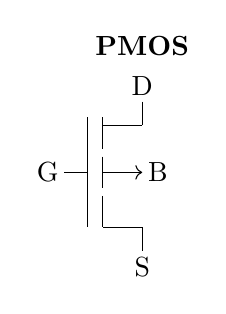
\begin{tikzpicture}[scale=1]
    % PMOS Enhancement
    \node at (0,2) {\textbf{PMOS}};
    \node at (0,1.5) {D};
    \draw (0,1.3) -- (0,1);
    \draw (0,1) -- (-0.5,1);
    
    % Broken channel
    \draw (-0.5,1.1) -- (-0.5,0.7);
    \draw (-0.5,0.6) -- (-0.5,0.2);
    \draw (-0.5,0.1) -- (-0.5,-0.3);
    
    % Source
    \draw (0,-0.3) -- (-0.5,-0.3);
    \draw (0,-0.3) -- (0,-0.6);
    \node at (0,-0.8) {S};
    
    % Gate
    \draw (-0.7,1.1) -- (-0.7,-0.3);
    \draw (-0.7,0.4) -- (-1,0.4);
    \node at (-1.2,0.4) {G};
    
    % Body/Arrow
    \draw (-0.5,0.4) -- (0,0.4);
    \node at (0.2,0.4) {B};
    \draw[<-] (0,0.4) -- (-0.5,0.4); % Arrow OUT for PMOS
\end{tikzpicture}
&
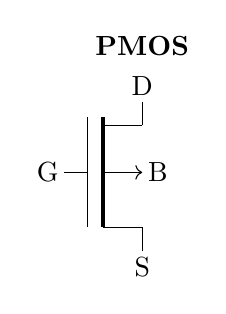
\begin{tikzpicture}[scale=1]
    % PMOS Depletion
    \node at (0,2) {\textbf{PMOS}};
    \node at (0,1.5) {D};
    \draw (0,1.3) -- (0,1);
    \draw (0,1) -- (-0.5,1);
    
    % Solid channel
    \draw[ultra thick] (-0.5,1.1) -- (-0.5,-0.3);
    
    % Source
    \draw (0,-0.3) -- (-0.5,-0.3);
    \draw (0,-0.3) -- (0,-0.6);
    \node at (0,-0.8) {S};
    
    % Gate
    \draw (-0.7,1.1) -- (-0.7,-0.3);
    \draw (-0.7,0.4) -- (-1,0.4);
    \node at (-1.2,0.4) {G};
    
    % Body/Arrow
    \draw (-0.5,0.4) -- (0,0.4);
    \node at (0.2,0.4) {B};
    \draw[<-] (0,0.4) -- (-0.5,0.4); % Arrow OUT for PMOS
\end{tikzpicture}
\\
\end{tabulary}
\end{center}

\textbf{Key Differences:}
\begin{itemize}
    \item \textbf{Enhancement}: Broken line represents no physical channel at $V_{GS}=0$.
    \item \textbf{Depletion}: Solid thick line represents existing physical channel at $V_{GS}=0$.
    \item \textbf{Arrows}: Inward for NMOS (p-substrate), Outward for PMOS (n-substrate).
\end{itemize}
\end{solutionbox}

\begin{mnemonicbox}
\mnemonic{Enhancement Needs voltage, Depletion has Default channel}
\end{mnemonicbox}

\questionmarks{1(b)}{4}{Define: 1) Hierarchy 2) Regularity}

\begin{solutionbox}
\textbf{Definitions:}

\begin{center}
\begin{tabulary}{\linewidth}{|L|L|L|}
\hline
\textbf{Term} & \textbf{Definition} & \textbf{Application} \\ \hline
\textbf{Hierarchy} & Top-down design approach where complex systems are broken into smaller, manageable modules. & Used in VLSI design flow from system level to transistor level. \\ \hline
\textbf{Regularity} & Design technique using repeated identical structures to reduce complexity. & Memory arrays, processor datapaths use regular structures. \\ \hline
\end{tabulary}
\end{center}

\textbf{Key Points:}
\begin{itemize}
    \item \textbf{Hierarchy benefits}: Easier design verification, modular testing, team collaboration.
    \item \textbf{Regularity advantages}: Reduced design time, better yield, simplified layout.
    \item \textbf{Design flow}: System $\rightarrow$ Behavioral $\rightarrow$ RTL $\rightarrow$ Gate $\rightarrow$ Layout.
\end{itemize}
\end{solutionbox}

\begin{mnemonicbox}
\mnemonic{Hierarchy Helps organize, Regularity Reduces complexity}
\end{mnemonicbox}

\questionmarks{1(c)}{7}{Explain MOS under external bias.}

\begin{solutionbox}
\textbf{MOS Bias Conditions:}

\begin{center}
\begin{tabulary}{\linewidth}{|L|L|L|L|}
\hline
\textbf{Bias Condition} & \textbf{Gate Voltage} & \textbf{Channel Formation} & \textbf{Current Flow} \\ \hline
\textbf{Accumulation} & $V_G < 0$ (NMOS) & Majority carriers accumulate & No channel \\ \hline
\textbf{Depletion} & $0 < V_G < V_T$ & Depletion region forms & Minimal current \\ \hline
\textbf{Inversion} & $V_G > V_T$ & Minority carriers form channel & Channel conducts \\ \hline
\end{tabulary}
\end{center}

\textbf{Operation Flow:}

\begin{center}
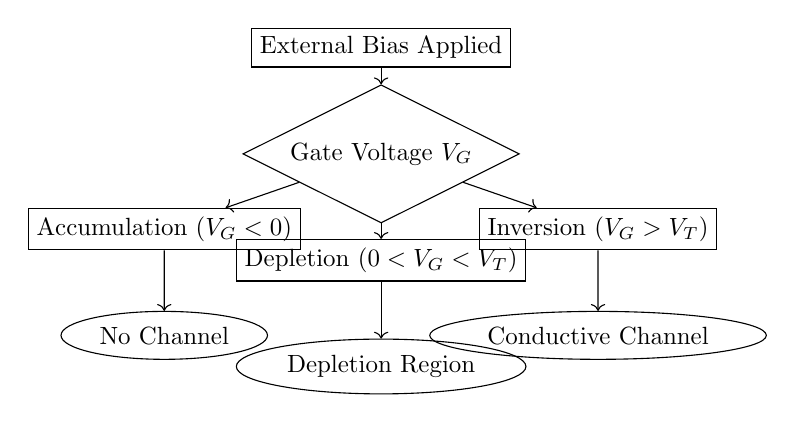
\begin{tikzpicture}[node distance=1.5cm, auto, scale=0.9, transform shape]
    \node (bias) [draw, rectangle] {External Bias Applied};
    \node (gate) [draw, diamond, below of=bias, aspect=2] {Gate Voltage $V_G$};
    
    \node (acc) [draw, rectangle, below left of=gate, xshift=-2cm] {Accumulation ($V_G < 0$)};
    \node (dep) [draw, rectangle, below of=gate] {Depletion ($0 < V_G < V_T$)};
    \node (inv) [draw, rectangle, below right of=gate, xshift=2cm] {Inversion ($V_G > V_T$)};
    
    \node (nochan) [draw, ellipse, below of=acc] {No Channel};
    \node (depreg) [draw, ellipse, below of=dep] {Depletion Region};
    \node (cond) [draw, ellipse, below of=inv] {Conductive Channel};
    
    \draw[->] (bias) -- (gate);
    \draw[->] (gate) -- (acc);
    \draw[->] (gate) -- (dep);
    \draw[->] (gate) -- (inv);
    \draw[->] (acc) -- (nochan);
    \draw[->] (dep) -- (depreg);
    \draw[->] (inv) -- (cond);
\end{tikzpicture}
\captionof{figure}{MOS Operating Modes}
\end{center}

\textbf{Key Concepts:}
\begin{itemize}
    \item \textbf{Band bending}: External voltage bends energy bands at oxide-silicon interface.
    \item \textbf{Threshold voltage ($V_T$)}: Minimum gate voltage needed for channel formation.
    \item \textbf{Inversion}: When surface potential $\phi_s = 2\phi_F$, strict inversion occurs.
\end{itemize}
\end{solutionbox}

\begin{mnemonicbox}
\mnemonic{Accumulation Attracts, Depletion Depletes, Inversion Inverts carriers}
\end{mnemonicbox}

\questionmarks{1(c) OR}{7}{What is the need for scaling? Explain types of scaling with its effect.}

\begin{solutionbox}
\textbf{Need for Scaling:}

\begin{center}
\begin{tabulary}{\linewidth}{|L|L|L|}
\hline
\textbf{Parameter} & \textbf{Benefit} & \textbf{Impact} \\ \hline
\textbf{Area reduction} & More transistors per chip & Higher integration density \\ \hline
\textbf{Speed increase} & Reduced delays & Better performance \\ \hline
\textbf{Power reduction} & Lower power consumption & Portable devices \\ \hline
\textbf{Cost reduction} & Cheaper per function & Market competitiveness \\ \hline
\end{tabulary}
\end{center}

\textbf{Types of Scaling:}

\begin{center}
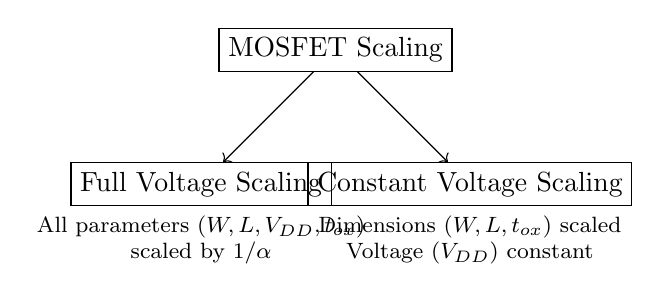
\begin{tikzpicture}[scale=0.9]
    \node (scal) [draw, rectangle] {MOSFET Scaling};
    \node (full) [draw, rectangle, below left of=scal, xshift=-1cm, yshift=-1cm] {Full Voltage Scaling};
    \node (const) [draw, rectangle, below right of=scal, xshift=1cm, yshift=-1cm] {Constant Voltage Scaling};
    
    \draw[->] (scal) -- (full);
    \draw[->] (scal) -- (const);
    
    \node [anchor=north, align=center, font=\footnotesize] at (full.south) {All parameters ($W, L, V_{DD}, t_{ox}$)\\scaled by $1/\alpha$};
    \node [anchor=north, align=center, font=\footnotesize] at (const.south) {Dimensions ($W, L, t_{ox}$) scaled\\Voltage ($V_{DD}$) constant};
\end{tikzpicture}
\end{center}

\textbf{Scaling Effects:}
\begin{itemize}
    \item \textbf{Full voltage scaling}: Maintains constant electric field. Power density remains constant.
    \item \textbf{Constant voltage scaling}: Electric field increases. Power density increases significantly.
\end{itemize}
\end{solutionbox}

\begin{mnemonicbox}
\mnemonic{Scaling Saves Space, Speed, and Spending}
\end{mnemonicbox}

\questionmarks{2(a)}{3}{Write short note on FPGA.}

\begin{solutionbox}
\textbf{FPGA Characteristics:}

\begin{center}
\begin{tabulary}{\linewidth}{|L|L|L|}
\hline
\textbf{Feature} & \textbf{Description} & \textbf{Advantage} \\ \hline
\textbf{Field Programmable} & Configurable after manufacturing & Flexibility in design \\ \hline
\textbf{Gate Array} & Array of logic blocks & Parallel processing \\ \hline
\textbf{Reconfigurable} & Can be reprogrammed & Prototype development \\ \hline
\end{tabulary}
\end{center}

\textbf{Details:}
\begin{itemize}
    \item \textbf{Applications}: Digital signal processing, embedded systems, prototyping.
    \item \textbf{Architecture}: Matrix of CLBs (Configurable Logic Blocks) connected by programmable routing.
    \item \textbf{Programming}: Typically SRAM-based (volatile) or Flash/Antifuse based.
\end{itemize}
\end{solutionbox}

\begin{mnemonicbox}
\mnemonic{FPGA: Flexible Programming for Gate Arrays}
\end{mnemonicbox}

\questionmarks{2(b)}{4}{Compare semi-custom and full custom design methodologies.}

\begin{solutionbox}
\textbf{Comparison:}

\begin{center}
\begin{tabulary}{\linewidth}{|L|L|L|}
\hline
\textbf{Parameter} & \textbf{Semi-Custom} & \textbf{Full Custom} \\ \hline
\textbf{Design Time} & Shorter (weeks) & Longer (months) \\ \hline
\textbf{Cost} & Lower development cost & Higher development cost \\ \hline
\textbf{Performance} & Moderate performance & Highest performance \\ \hline
\textbf{Area Efficiency} & Less efficient & Most efficient \\ \hline
\textbf{Applications} & ASICs, moderate volume & Microprocessors, high volume \\ \hline
\textbf{Design Effort} & Standard cells used & Every transistor designed manually \\ \hline
\end{tabulary}
\end{center}
\end{solutionbox}

\begin{mnemonicbox}
\mnemonic{Semi-custom is Standard, Full custom is Finest}
\end{mnemonicbox}

\questionmarks{2(c)}{7}{Explain MOSFET operation for 1) $0 < V_{DS} < V_{DSAT}$ 2) $V_{DS} = V_{DSAT}$ 3) $V_{DS} > V_{DSAT}$}

\begin{solutionbox}
\textbf{Operating Regions:}

\begin{center}
\begin{tabulary}{\linewidth}{|L|L|L|L|}
\hline
\textbf{Region} & \textbf{Condition} & \textbf{Channel State} & \textbf{Current ($I_D$)} \\ \hline
\textbf{Linear} & $V_{DS} < V_{DSAT}$ & Uniform continuous channel & $\propto V_{DS}$ \\ \hline
\textbf{Saturation Onset} & $V_{DS} = V_{DSAT}$ & Pinch-off begins at drain & Max linear current \\ \hline
\textbf{Saturation} & $V_{DS} > V_{DSAT}$ & Pinched off channel & Constant \\ \hline
\end{tabulary}
\end{center}

\textbf{Diagrammatic Representation:}

\begin{center}
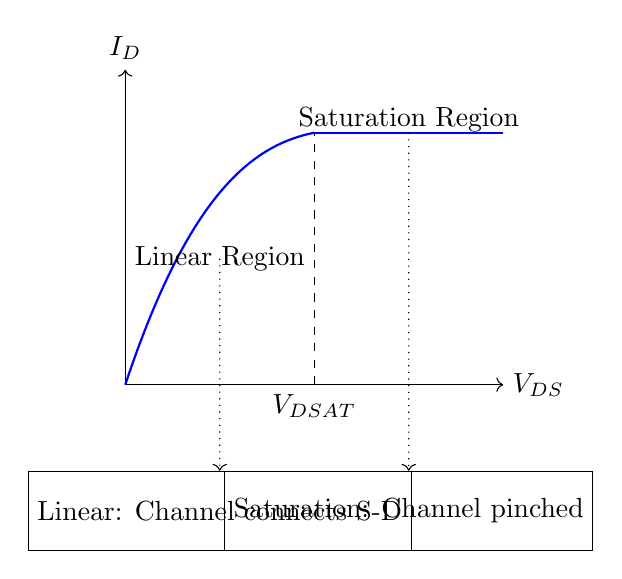
\begin{tikzpicture}[scale=0.8]
    % Axes
    \draw[->] (0,0) -- (6,0) node[right] {$V_{DS}$};
    \draw[->] (0,0) -- (0,5) node[above] {$I_D$};
    
    % Curve
    \draw[thick, blue] (0,0) .. controls (1,3) and (2,3.8) .. (3,4); % Linear
    \draw[thick, blue] (3,4) -- (6,4); % Saturation
    
    % Points
    \draw[dashed] (3,0) -- (3,4);
    \node[below] at (3,0) {$V_{DSAT}$};
    
    \node at (1.5, 2) {Linear Region};
    \node at (4.5, 4.2) {Saturation Region};
    
    % Channel visual
    \node[draw, rectangle, minimum width=2cm, minimum height=1cm] (lin) at (1.5,-2) {Linear: Channel connects S-D};
    \node[draw, rectangle, minimum width=2cm, minimum height=1cm] (sat) at (4.5,-2) {Saturation: Channel pinched};
    
    \draw[->, dotted] (1.5, 2) -- (lin);
    \draw[->, dotted] (4.5, 4) -- (sat);
\end{tikzpicture}
\captionof{figure}{MOSFET I-V Characteristic}
\end{center}

\textbf{Analysis:}
\begin{itemize}
    \item \textbf{Linearn Region}: Channel behaves as a voltage-controlled resistor. $I_D$ increases linearly with $V_{DS}$.
    \item \textbf{Saturation Region}: Channel is pinched off at drain end. Current flow is due to electric field drift across depletion region. $I_D$ becomes independent of $V_{DS}$ (ignoring channel length modulation).
    \item \textbf{$V_{DSAT}$}: Saturation voltage, typically $V_{GS} - V_T$.
\end{itemize}
\end{solutionbox}

\begin{mnemonicbox}
\mnemonic{Linear Likes VDS, Saturation Says no more}
\end{mnemonicbox}

\questionmarks{2(a) OR}{3}{Explain standard cell-based design.}

\begin{solutionbox}
\textbf{Overview:}

\begin{center}
\begin{tabulary}{\linewidth}{|L|L|L|}
\hline
\textbf{Component} & \textbf{Description} & \textbf{Benefit} \\ \hline
\textbf{Standard Cells} & Pre-designed logic gates (AND, OR, FF) & Faster design cycle \\ \hline
\textbf{Cell Library} & Collection of characterized cells with physical layouts & Predictable performance \\ \hline
\textbf{Place \& Route} & Automated layout generation using tools & Reduced manual effort \\ \hline
\end{tabulary}
\end{center}

\textbf{Design Flow:}
\begin{itemize}
    \item Logic Synthesis $\rightarrow$ Placement $\rightarrow$ Routing $\rightarrow$ Verification.
    \item EDA tools handle the complex physical implementation.
    \item Provides a balance between performance, area, and power.
\end{itemize}
\end{solutionbox}

\begin{mnemonicbox}
\mnemonic{Standard Cells Speed up Synthesis}
\end{mnemonicbox}

\questionmarks{2(b) OR}{4}{Draw and explain Y-chart.}

\begin{solutionbox}
\textbf{Gajski-Kuhn Y-Chart:}

\begin{center}
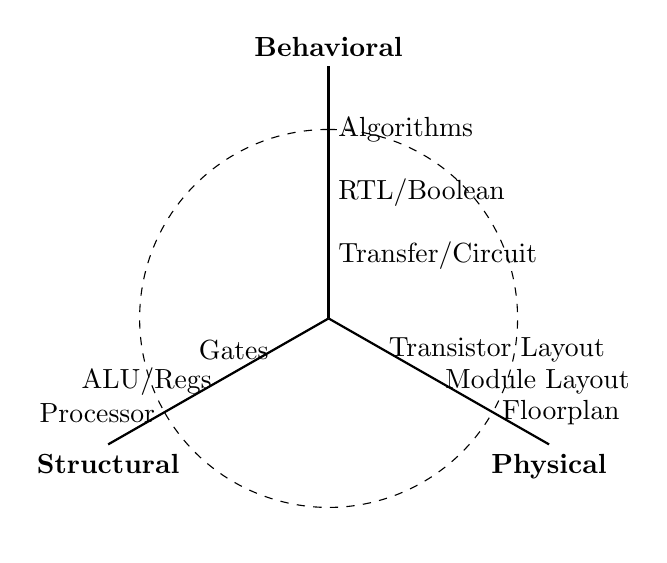
\begin{tikzpicture}[scale=0.8]
    % Axes
    \draw[thick] (0,0) -- (0,4) node[above] {\textbf{Behavioral}};
    \draw[thick] (0,0) -- (-3.5,-2) node[below] {\textbf{Structural}};
    \draw[thick] (0,0) -- (3.5,-2) node[below] {\textbf{Physical}};
    
    % Concentric Circles (Arcs)
    \draw[dashed] (0,3) arc (90:210:3);
    \draw[dashed] (0,3) arc (90:-30:3);
    \draw[dashed] (-2.6,-1.5) arc (210:330:3);
    
    % Labels
    \node[anchor=west] at (0,3) {Algorithms};
    \node[anchor=west] at (0,2) {RTL/Boolean};
    \node[anchor=west] at (0,1) {Transfer/Circuit};
    
    \node[anchor=east] at (-2.6,-1.5) {Processor};
    \node[anchor=east] at (-1.7,-1) {ALU/Regs};
    \node[anchor=east] at (-0.8,-0.5) {Gates};
    
    \node[anchor=west] at (2.6,-1.5) {Floorplan};
    \node[anchor=west] at (1.7,-1) {Module Layout};
    \node[anchor=west] at (0.8,-0.5) {Transistor Layout};
\end{tikzpicture}
\captionof{figure}{Y-Chart Representation}
\end{center}

\textbf{Domains:}
\begin{itemize}
    \item \textbf{Behavioral}: Describes \textit{what} the system does (Functionality).
    \item \textbf{Structural}: Describes \textit{how} components are interconnected.
    \item \textbf{Physical}: Describes the \textit{geometry} and layout of the implementation.
\end{itemize}
\end{solutionbox}

\begin{mnemonicbox}
\mnemonic{Y-chart: behaVior, Structure, PhYsical}
\end{mnemonicbox}

\questionmarks{2(c) OR}{7}{Explain gradual channel approximation for MOSFET current-voltage characteristics.}

\begin{solutionbox}
\textbf{Gradual Channel Approximation (GCA):}

\textbf{Assumptions:}
\begin{center}
\begin{tabulary}{\linewidth}{|L|L|L|}
\hline
\textbf{Assumption} & \textbf{Description} & \textbf{Justification} \\ \hline
\textbf{Gradual Channel} & Variation of field along channel ($y$) $\ll$ variation perpendicular ($x$). & Valid for long channel devices ($L \gg t_{ox}$). \\ \hline
\textbf{1D Analysis} & Current flows mainly in $y$-direction (source to drain). & Simplifies potential analysis. \\ \hline
\textbf{Drift Current} & Diffusion current is neglected. & Dominant mechanism in strong inversion. \\ \hline
\end{tabulary}
\end{center}

\textbf{Derivation Summary:}
\begin{itemize}
    \item Induced charge density: $Q_n(y) = -C_{ox}[V_{GS} - V(y) - V_T]$.
    \item Drain Current: $I_D = -W \mu_n Q_n(y) \frac{dV}{dy}$.
    \item Integrating from $y=0$ to $L$ and $V=0$ to $V_{DS}$:
    \[ I_D = \mu_n C_{ox} \frac{W}{L} \left[ (V_{GS}-V_T)V_{DS} - \frac{V_{DS}^2}{2} \right] \]
\end{itemize}

\textbf{Limitations:}
\begin{itemize}
    \item \textbf{Short Channel Effects}: GCA fails when $L$ is comparable to depletion widths.
    \item \textbf{Velocity Saturation}: Carrier velocity doesn't increase linearly with high fields.
\end{itemize}
\end{solutionbox}

\begin{mnemonicbox}
\mnemonic{Gradual change Gives simple Gain equations}
\end{mnemonicbox}

\questionmarks{3(a)}{3}{Draw symbol and write truth table of ideal inverter. Draw and explain VTC of ideal inverter.}

\begin{solutionbox}
\textbf{Ideal Inverter:}

\begin{center}
\begin{tabulary}{\linewidth}{C C}
\textbf{Symbol} & \textbf{Truth Table} \\
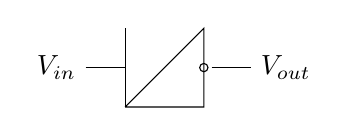
\begin{tikzpicture}[scale=1]
    % Inverter Symbol
    \draw (0,0) -- (1,0) -- (1,1) -- (0,0); % Triangle
    \draw (0,1) -- (0,0);
    \draw (1,0.5) circle (1.5pt); % Bubble
    \draw (-0.5,0.5) -- (0,0.5); % Input
    \node[left] at (-0.5,0.5) {$V_{in}$};
    \draw (1.1,0.5) -- (1.6,0.5); % Output
    \node[right] at (1.6,0.5) {$V_{out}$};
\end{tikzpicture}
&
\begin{tabular}{|c|c|}
\hline
$V_{in}$ & $V_{out}$ \\ \hline
$0$ & $1 (V_{DD})$ \\ \hline
$1 (V_{DD})$ & $0$ \\ \hline
\end{tabular}
\\
\end{tabulary}
\end{center}

\textbf{Voltage Transfer Characteristic (VTC):}

\begin{center}
\begin{tikzpicture}[scale=0.8]
    \draw[->] (0,0) -- (4,0) node[right] {$V_{in}$};
    \draw[->] (0,0) -- (0,4) node[above] {$V_{out}$};
    
    \node[left] at (0,3.5) {$V_{DD}$};
    \node[below] at (3.5,0) {$V_{DD}$};
    \node[below] at (1.75,0) {$V_{DD}/2$};
    
    % Ideal curve
    \draw[blue, thick] (0,3.5) -- (1.75,3.5) -- (1.75,0) -- (3.5,0);
    
    \draw[dashed] (1.75,0) -- (1.75,3.5);
\end{tikzpicture}
\captionof{figure}{Ideal VTC}
\end{center}

\textbf{Characteristics:}
\begin{itemize}
    \item Infinite gain at switching threshold ($V_{DD}/2$).
    \item Noise margins $NM_H = NM_L = V_{DD}/2$.
    \item Zero power consumption in steady states.
\end{itemize}
\end{solutionbox}

\begin{mnemonicbox}
\mnemonic{Ideal Inverter: Infinite gain, Instant switching}
\end{mnemonicbox}

\questionmarks{3(b)}{4}{Explain generalized inverter circuit with its VTC.}

\begin{solutionbox}
\textbf{Generalized Inverter Structure:}

\begin{center}
\begin{tabulary}{\linewidth}{L L}
\textbf{Components:} & \textbf{Circuit:} \\
1. \textbf{Driver}: Pull-down NMOS transistor. & 
\multirow{3}{*}{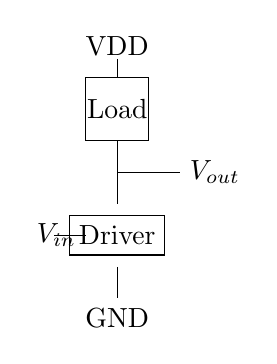
\begin{tikzpicture}[scale=0.8]
    \node at (0,3) {VDD};
    \draw (0,2.8) -- (0,2.5);
    \draw (-0.5,2.5) rectangle (0.5,1.5);
    \node at (0,2) {Load};
    \draw (0,1.5) -- (0,1);
    \draw (0,1) -- (1,1) node[right] {$V_{out}$};
    
    \draw (0,1) -- (0,0.5);
    \node[draw,rectangle,minimum size=0.5cm] (n) at (0,0) {Driver};
    \draw (-1,0) -- (-0.5,0) node[left] {$V_{in}$};
    \draw (0,-0.5) -- (0,-1) node[below] {GND};
\end{tikzpicture}} \\
2. \textbf{Load}: Pull-up device (Resistor/Transistor). & \\
3. \textbf{Operation}: Input separates driver ON/OFF states. & \\
\end{tabulary}
\end{center}

\textbf{VTC Regions:}
\begin{itemize}
    \item \textbf{Region 1 (High Output)}: $V_{in} < V_T$. Driver OFF, Load pulls up to $V_{OH} \approx V_{DD}$.
    \item \textbf{Region 2 (Transition)}: Both devices conducting. Voltage drops sharply.
    \item \textbf{Region 3 (Low Output)}: $V_{in}$ High. Driver ON (Linear). $V_{out} = V_{OL}$.
\end{itemize}
\end{solutionbox}

\begin{mnemonicbox}
\mnemonic{Generalized design: Driver pulls Down, Load lifts Up}
\end{mnemonicbox}

\questionmarks{3(c)}{7}{Describe depletion load nMOS inverter with its circuit, operating region and VTC.}

\begin{solutionbox}
\textbf{Depletion Load NMOS Inverter:}

\begin{center}
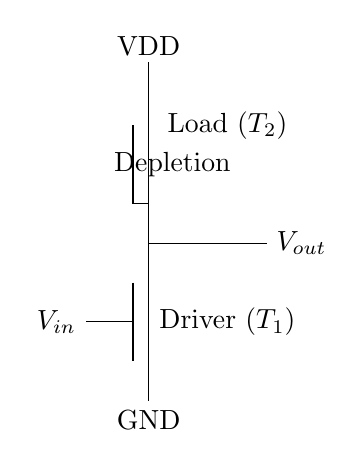
\begin{tikzpicture}[scale=1]
    \node at (0,4.5) {VDD};
    \draw (0,4.3) -- (0,4);
    
    % Depletion Load
    \draw (0,4) -- (0,3.5);
    \draw (0,3.5) -- (0,2.5); % Channel
    \draw (-0.2,3.5) -- (-0.2,2.5); % Gate
    \draw (0.3,3) node {Depletion};
    \draw (-0.2,2.5) -- (0,2.5); % Short gate to source (Vgs=0)
    \draw (0,2.5) -- (0,2);
    
    % Output
    \draw (0,2) -- (1.5,2) node[right] {$V_{out}$};
    
    % Driver (Enhancement)
    \draw (0,2) -- (0,1.5);
    \draw (0,1.5) -- (0,0.5); % Channel
    \draw (-0.2,1.5) -- (-0.2,0.5); % Gate
    \draw (-0.2,1) -- (-0.8,1) node[left] {$V_{in}$};
    \draw (0,0.5) -- (0,0) node[below] {GND};
    
    \node at (1,3.5) {Load ($T_2$)};
    \node at (1,1) {Driver ($T_1$)};
\end{tikzpicture}
\captionof{figure}{Depletion Load Inverter Circuit}
\end{center}

\textbf{Operating Regions:}
\begin{center}
\begin{tabulary}{\linewidth}{|L|L|L|L|}
\hline
\textbf{Input State} & \textbf{Driver ($T_1$)} & \textbf{Load ($T_2$)} & \textbf{Output} \\ \hline
$V_{in} < V_{TN}$ (Low) & OFF (Cutoff) & ON (Linear) & $V_{OH} = V_{DD}$ \\ \hline
$V_{in}$ Trans. & Saturation & Saturation & Falling \\ \hline
$V_{in} > V_{IH}$ (High) & ON (Linear) & ON (Saturation) & $V_{OL}$ (Small) \\ \hline
\end{tabulary}
\end{center}

\textbf{VTC Characteristics:}
\begin{itemize}
    \item \textbf{High Output}: Full $V_{DD}$ because depletion load pulls up fully.
    \item \textbf{Transition}: Sharp, providing good noise margins.
    \item \textbf{Low Output}: Non-zero $V_{OL} \approx 0$ (Ratioed logic).
\end{itemize}
\end{solutionbox}

\begin{mnemonicbox}
\mnemonic{Depletion Device Delivers Decent drive}
\end{mnemonicbox}

\questionmarks{3(a) OR}{3}{Explain noise margin.}

\begin{solutionbox}
\textbf{Definition:}
Noise Margin is the maximum noise voltage added to an input signal that does not cause a change in the logic state of the output. It measures noise immunity.

\textbf{Parameters:}
\begin{center}
\begin{tabulary}{\linewidth}{|L|L|L|}
\hline
\textbf{Parameter} & \textbf{Formula} & \textbf{Description} \\ \hline
\textbf{NMH} & $V_{OH} - V_{IH}$ & High Noise Margin \\ \hline
\textbf{NML} & $V_{IL} - V_{OL}$ & Low Noise Margin \\ \hline
$V_{OH}$ & - & Min Output High Voltage \\ \hline
$V_{OL}$ & - & Max Output Low Voltage \\ \hline
$V_{IH}$ & - & Min Input High Voltage \\ \hline
$V_{IL}$ & - & Max Input Low Voltage \\ \hline
\end{tabulary}
\end{center}
\end{solutionbox}

\begin{mnemonicbox}
\mnemonic{Noise Margins Maintain signal integrity}
\end{mnemonicbox}

\questionmarks{3(b) OR}{4}{Explain resistive load inverter.}

\begin{solutionbox}
\textbf{Circuit and Analysis:}

\begin{center}
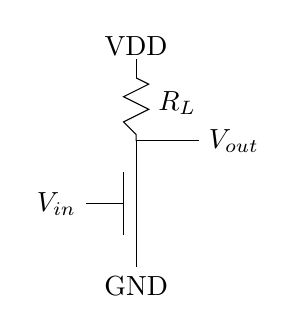
\begin{tikzpicture}[scale=0.8]
    \node at (0,3) {VDD};
    \draw (0,2.8) -- (0,2.5);
    % Resistor
    \draw (0,2.5) -- (0.2,2.4) -- (-0.2,2.2) -- (0.2,2.0) -- (-0.2,1.8) -- (0,1.6) -- (0,1.5);
    \node[right] at (0.2, 2.1) {$R_L$};
    
    \draw (0,1.5) -- (1,1.5) node[right] {$V_{out}$};
    \draw (0,1.5) -- (0,1);
    
    % NMOS
    \draw (0,1) -- (0,0);
    \draw (-0.2,1) -- (-0.2,0);
    \draw (-0.2,0.5) -- (-0.8,0.5) node[left] {$V_{in}$};
    
    \draw (0,0) -- (0,-0.5) node[below] {GND};
\end{tikzpicture}
\captionof{figure}{Resistive Load Inverter}
\end{center}

\textbf{Operation:}
\begin{itemize}
    \item \textbf{Input Low}: NMOS OFF. Output pulled to $V_{DD}$ through $R_L$.
    \item \textbf{Input High}: NMOS ON. Current flows through $R_L$ and NMOS. Output $V_{OL} = V_{DD} \frac{R_{MN}}{R_{MN} + R_L}$.
\end{itemize}

\textbf{Drawbacks:}
\begin{itemize}
    \item Large area required for resistor on-chip.
    \item Static power consumption when output is low ($V_{DD}^2/R_L$).
\end{itemize}
\end{solutionbox}

\begin{mnemonicbox}
\mnemonic{Resistor Restricts current, Reduces performance}
\end{mnemonicbox}

\questionmarks{3(c) OR}{7}{Explain CMOS inverter with its VTC.}

\begin{solutionbox}
\textbf{CMOS Inverter:}

\begin{center}
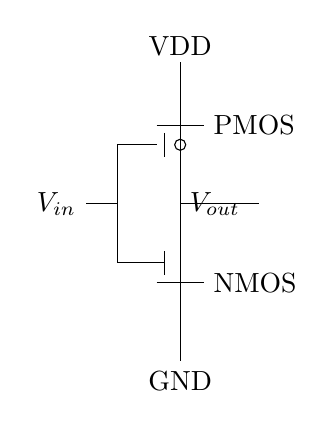
\begin{tikzpicture}[scale=1]
    \node at (0,3.5) {VDD};
    \draw (0,3.3) -- (0,3);
    
    % PMOS
    \draw (0,3) -- (0,2.5);
    \draw (-0.3,2.5) -- (0.3,2.5); % Source
    \draw (0,2.5) -- (0,2); % Drain
    \draw (-0.2,2.4) -- (-0.2,2.1); % Gate
    \draw (0,2.25) circle (2pt); % Bubble
    \draw (-0.3,2.25) -- (-0.8,2.25); % Gate connection
    \node[right] at (0.3,2.5) {PMOS};

    % Output
    \draw (0,2) -- (0,1) node[midway, right] {$V_{out}$};
    \draw (0,1.5) -- (1,1.5);

    % NMOS
    \draw (0,1) -- (0,0.5); % Drain
    \draw (-0.3,0.5) -- (0.3,0.5);
    \draw (0,0.5) -- (0,0); % Source
    \draw (-0.2,0.9) -- (-0.2,0.6); % Gate
    \draw (-0.2,0.75) -- (-0.8,0.75); % Gate connection
    \node[right] at (0.3,0.5) {NMOS};

    \draw (0,0) -- (0,-0.5) node[below] {GND};
    
    % Input join
    \draw (-0.8,2.25) -- (-0.8,0.75);
    \draw (-0.8,1.5) -- (-1.2,1.5) node[left] {$V_{in}$};
\end{tikzpicture}
\captionof{figure}{CMOS Inverter Circuit}
\end{center}

\textbf{VTC Regions \& Operation:}
\begin{center}
\begin{tabulary}{\linewidth}{|L|L|L|L|L|}
\hline
\textbf{Region} & \textbf{Input Range} & \textbf{PMOS} & \textbf{NMOS} & \textbf{Output} \\ \hline
\textbf{1} & $V_{in} < V_{TN}$ & ON (Linear) & OFF & $V_{DD}$ \\ \hline
\textbf{2} & $V_{TN} < V_{in} < V_{DD}/2$ & ON (Lin) & ON (Sat) & High Drop \\ \hline
\textbf{3} & $V_{in} \approx V_{DD}/2$ & Saturation & Saturation & Switch \\ \hline
\textbf{4} & $V_{DD}/2 < V_{in} < V_{DD}+V_{TP}$ & ON (Sat) & ON (Lin) & Low Drop \\ \hline
\textbf{5} & $V_{in} > V_{DD}+V_{TP}$ & OFF & ON (Linear) & $0$ \\ \hline
\end{tabulary}
\end{center}

\textbf{Advantages:} - Zero static power. - Full rail-to-rail logic swing. - High noise margins.
\end{solutionbox}

\begin{mnemonicbox}
\mnemonic{CMOS: Complementary for Complete performance}
\end{mnemonicbox}


\questionmarks{4(a)}{3}{Draw AOI with CMOS implementation.}

\begin{solutionbox}
\textbf{AOI Logic:} $Y = \overline{AB + CD}$

\textbf{CMOS Implementation:}

\begin{center}
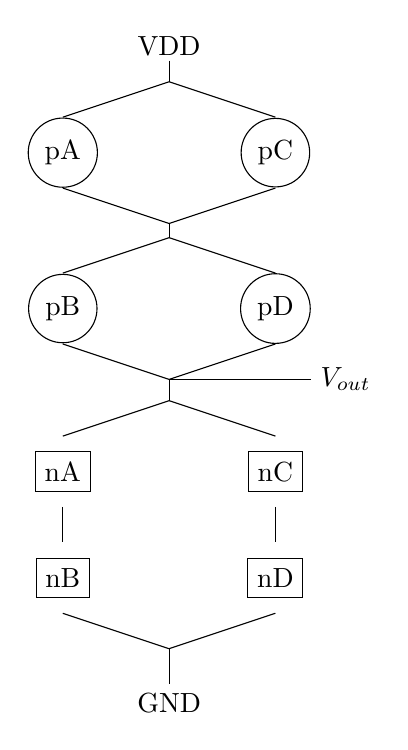
\begin{tikzpicture}[scale=0.9]
    \node at (0,5.5) {VDD};
    \draw (0,5.3) -- (0,5);
    
    % PUN (Dual): (A'+B')(C'+D')
    \draw (0,5) -- (-1.5,4.5);
    \draw (0,5) -- (1.5,4.5);
    
    \node[draw,circle,minimum size=0.5cm] (pA) at (-1.5,4) {pA};
    \node[draw,circle,minimum size=0.5cm] (pC) at (1.5,4) {pC};
    \draw (-1.5,3.5) -- (0,3);
    \draw (1.5,3.5) -- (0,3);
    
    \draw (0,3) -- (0,2.8);
    \draw (0,2.8) -- (-1.5,2.3);
    \draw (0,2.8) -- (1.5,2.3);
    
    \node[draw,circle,minimum size=0.5cm] (pB) at (-1.5,1.8) {pB};
    \node[draw,circle,minimum size=0.5cm] (pD) at (1.5,1.8) {pD};
    \draw (-1.5,1.3) -- (0,0.8);
    \draw (1.5,1.3) -- (0,0.8);
    
    % Output
    \draw (0,0.8) -- (2,0.8) node[right] {$V_{out}$};
    \draw (0,0.8) -- (0,0.5);
    
    % PDN: AB + CD
    \draw (0,0.5) -- (-1.5,0);
    \draw (0,0.5) -- (1.5,0);
    
    \node[draw,rectangle,minimum size=0.5cm] (nA) at (-1.5,-0.5) {nA};
    \draw (-1.5,-1) -- (-1.5,-1.5);
    \node[draw,rectangle,minimum size=0.5cm] (nB) at (-1.5,-2) {nB};
    
    \node[draw,rectangle,minimum size=0.5cm] (nC) at (1.5,-0.5) {nC};
    \draw (1.5,-1) -- (1.5,-1.5);
    \node[draw,rectangle,minimum size=0.5cm] (nD) at (1.5,-2) {nD};
    
    \draw (-1.5,-2.5) -- (0,-3);
    \draw (1.5,-2.5) -- (0,-3);
    \draw (0,-3) -- (0,-3.5) node[below] {GND};
\end{tikzpicture}
\captionof{figure}{AOI CMOS Circuit}
\end{center}
\end{solutionbox}

\begin{mnemonicbox}
\mnemonic{AOI: AND-OR then Invert}
\end{mnemonicbox}

\questionmarks{4(b)}{4}{Implement two input NOR and NAND gate using depletion load nMOS.}

\begin{solutionbox}
\textbf{Depletion Load Gates:}

\begin{center}
\begin{tabulary}{\linewidth}{C C}
\textbf{NOR Gate} & \textbf{NAND Gate} \\
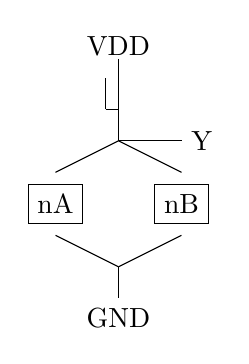
\begin{tikzpicture}[scale=0.8]
    \node at (0,4) {VDD};
    \draw (0,3.8) -- (0,3.5);
    \draw (0,3.5) -- (0,3); % Depletion Load
    \draw (-0.2,3) -- (-0.2,3.5); \draw (-0.2,3) -- (0,3);
    \draw (0,3) -- (0,2.5);
    \draw (0,2.5) -- (1,2.5) node[right] {Y};
    
    % Parallel NMOS A, B
    \draw (0,2.5) -- (-1,2);
    \draw (0,2.5) -- (1,2);
    \node[draw,rectangle,minimum size=0.5cm] (nA) at (-1,1.5) {nA};
    \node[draw,rectangle,minimum size=0.5cm] (nB) at (1,1.5) {nB};
    \draw (-1,1) -- (0,0.5);
    \draw (1,1) -- (0,0.5);
    \draw (0,0.5) -- (0,0) node[below] {GND};
\end{tikzpicture}
&
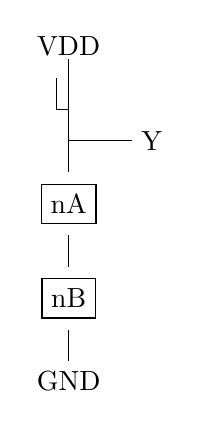
\begin{tikzpicture}[scale=0.8]
    \node at (0,4) {VDD};
    \draw (0,3.8) -- (0,3.5);
    \draw (0,3.5) -- (0,3); % Depletion Load
    \draw (-0.2,3) -- (-0.2,3.5); \draw (-0.2,3) -- (0,3);
    \draw (0,3) -- (0,2.5);
    \draw (0,2.5) -- (1,2.5) node[right] {Y};
    
    % Series NMOS A, B
    \draw (0,2.5) -- (0,2);
    \node[draw,rectangle,minimum size=0.5cm] (nA) at (0,1.5) {nA};
    \draw (0,1) -- (0,0.5);
    \node[draw,rectangle,minimum size=0.5cm] (nB) at (0,0) {nB};
    \draw (0,-0.5) -- (0,-1) node[below] {GND};
\end{tikzpicture}
\\
\end{tabulary}
\end{center}

\textbf{Truth Tables:}
\begin{center}
\begin{tabular}{|c|c|c|c|}
\hline
A & B & NOR & NAND \\ \hline
0 & 0 & 1 & 1 \\ \hline
0 & 1 & 0 & 1 \\ \hline
1 & 0 & 0 & 1 \\ \hline
1 & 1 & 0 & 0 \\ \hline
\end{tabular}
\end{center}
\end{solutionbox}

\begin{mnemonicbox}
\mnemonic{NOR needs None high, NAND Needs All high to be low}
\end{mnemonicbox}

\questionmarks{4(c)}{7}{Implement CMOS SR latch using NOR2 and NAND2 gates.}

\begin{solutionbox}
\textbf{SR Latch using NOR Gates:}

\begin{center}
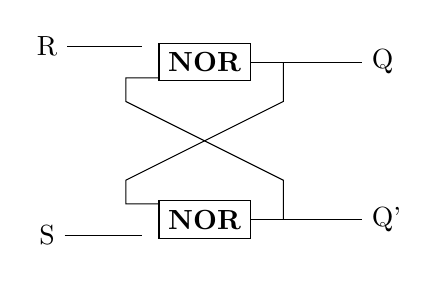
\begin{tikzpicture}[scale=1]
    \node[draw, rectangle] (nor1) at (0,2) {\textbf{NOR}};
    \node[draw, rectangle] (nor2) at (0,0) {\textbf{NOR}};
    
    \node (R) at (-2,2.2) {R};
    \node (S) at (-2,-0.2) {S};
    \draw (R) -- (-0.8,2.2); % Input R top
    \draw (S) -- (-0.8,-0.2); % Input S bot
    
    \draw (nor1.east) -- (2,2) node[right] {Q};
    \draw (nor2.east) -- (2,0) node[right] {Q'};
    
    % Feedback
    \draw (1,2) -- (1,1.5) -- (-1,0.5) -- (-1,0.2) -- (nor2.west |- 0,0.2);
    \draw (1,0) -- (1,0.5) -- (-1,1.5) -- (-1,1.8) -- (nor1.west |- 0,1.8);
\end{tikzpicture}
\captionof{figure}{SR Latch Logic Symbol}
\end{center}

\textbf{CMOS Implementation (NOR Latch):}
Two CMOS NOR2 gates with cross-coupled inputs.
\begin{itemize}
    \item \textbf{Top NOR}: Inputs R and Q'. Output Q.
    \item \textbf{Bottom NOR}: Inputs S and Q. Output Q'.
\end{itemize}

\textbf{State Table:}
\begin{center}
\begin{tabular}{|c|c|c|c|}
\hline
S & R & Q(n+1) & State \\ \hline
0 & 0 & Q(n) & Hold \\ \hline
0 & 1 & 0 & Reset \\ \hline
1 & 0 & 1 & Set \\ \hline
1 & 1 & 0 & Invalid \\ \hline
\end{tabular}
\end{center}
\end{solutionbox}

\begin{mnemonicbox}
\mnemonic{SR latch: Set-Reset with cross-coupled gates}
\end{mnemonicbox}

\questionmarks{4(a) OR}{3}{Implement XOR function using CMOS.}

\begin{solutionbox}
\textbf{XOR Function:} $Y = A \oplus B = A\bar{B} + \bar{A}B$.
\textbf{Inverted logic:} $\overline{Y} = \overline{A\bar{B} + \bar{A}B} = (A+B)(\bar{A}+\bar{B}) = XNOR$.
Usually XOR is implemented using 12 transistors (with inverters) or transmission gates (6-8 transistors).

\textbf{Static CMOS (12T):} Implement XNOR in PDN and invert, or XOR directly using complex gate.
Direct XOR PDN: Parallel (A series B') and (A' series B).
PUN: Series (A parallel B') and (A' parallel B).

\begin{center}
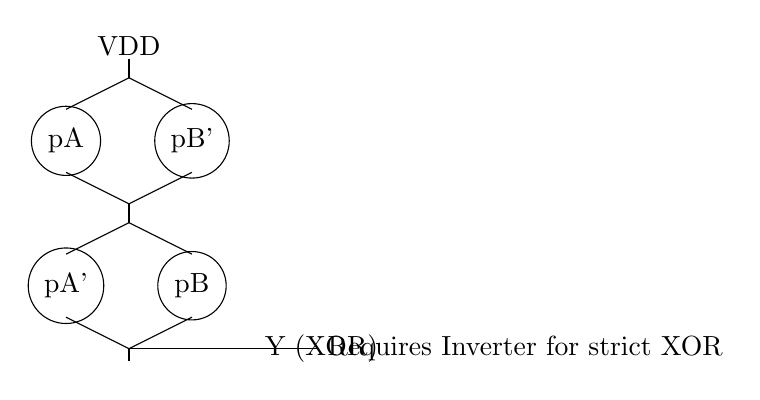
\begin{tikzpicture}[scale=0.8]
    \node at (0,5) {VDD};
    \draw (0,4.8) -- (0,4.5);
    
    % PUN logic: (A || B') series (A' || B)
    % Block 1: A || B'
    \draw (0,4.5) -- (-1,4); \draw (0,4.5) -- (1,4);
    \node[draw,circle,minimum size=0.5cm] (pA) at (-1,3.5) {pA};
    \node[draw,circle,minimum size=0.5cm] (pBb) at (1,3.5) {pB'};
    \draw (-1,3) -- (0,2.5); \draw (1,3) -- (0,2.5);
    
    \draw (0,2.5) -- (0,2.2);
    
    % Block 2: A' || B
    \draw (0,2.2) -- (-1,1.7); \draw (0,2.2) -- (1,1.7);
    \node[draw,circle,minimum size=0.5cm] (pAb) at (-1,1.2) {pA'};
    \node[draw,circle,minimum size=0.5cm] (pB) at (1,1.2) {pB};
    \draw (-1,0.7) -- (0,0.2); \draw (1,0.7) -- (0,0.2);
    
    \draw (0,0.2) -- (2,0.2) node[right] {Y (XOR)}; % Note: This logic structure produces XNOR actually, inversion needed for XOR from basic And-Or-Invert principles if strictly following bubbles. 
    % Let's clarify: Y = A (+) B. 
    % PDN needs to conduct when Y=0 (A=B). So PDN = AB + A'B'. This is XNOR.
    % So output of this stage is (XNOR)' = XOR.
    % Wait. PDN conducts for 0. So PDN implements Function_bar.
    % If we want Y=XOR. Y_bar = XNOR.
    % So PDN should implement XNOR: AB + A'B'.
    % PUN should implement XOR (dual).
    % My PUN above implements (A+B')(A'+B) = AA' + AB + A'B' + B'B = AB + A'B'. This is XNOR logic.
    % So PUN conducts when inputs match. Output High when inputs match => XNOR.
    % So this circuit is XNOR. To get XOR, invert output.
    
    \draw (2,0.2) -- (2.5,0.2) -- (3,0.2);
    \node[right] at (3,0.2) {Requires Inverter for strict XOR};
    
    \draw (0,0.2) -- (0,0);
\end{tikzpicture}
\captionof{figure}{CMOS Structure (Logic Analysis)}
\end{center}
\textit{Note: Standard static CMOS XOR requires identifying $\bar{Y} = XNOR = AB + \bar{A}\bar{B}$. The PDN implements $AB + \bar{A}\bar{B}$. The PUN is dual.}
\end{solutionbox}

\begin{mnemonicbox}
\mnemonic{XOR: eXclusive OR, different inputs give 1}
\end{mnemonicbox}

\questionmarks{4(b) OR}{4}{Implement two input NOR and NAND gate using CMOS.}

\begin{solutionbox}
\textbf{CMOS Gates:}

\begin{center}
\begin{tabulary}{\linewidth}{C C}
\textbf{NAND Gate} & \textbf{NOR Gate} \\
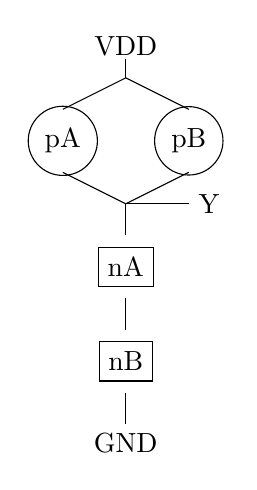
\begin{tikzpicture}[scale=0.8]
    % NAND
    \node at (0,4) {VDD};
    \draw (0,3.8) -- (0,3.5);
    % PUN Parallel
    \draw (0,3.5) -- (-1,3); \draw (0,3.5) -- (1,3);
    \node[draw,circle,minimum size=0.5cm] (pA) at (-1,2.5) {pA};
    \node[draw,circle,minimum size=0.5cm] (pB) at (1,2.5) {pB};
    \draw (-1,2) -- (0,1.5); \draw (1,2) -- (0,1.5);
    \draw (0,1.5) -- (1,1.5) node[right] {Y};
    % PDN Series
    \draw (0,1.5) -- (0,1);
    \node[draw,rectangle,minimum size=0.5cm] (nA) at (0,0.5) {nA};
    \draw (0,0) -- (0,-0.5);
    \node[draw,rectangle,minimum size=0.5cm] (nB) at (0,-1) {nB};
    \draw (0,-1.5) -- (0,-2) node[below] {GND};
\end{tikzpicture}
&
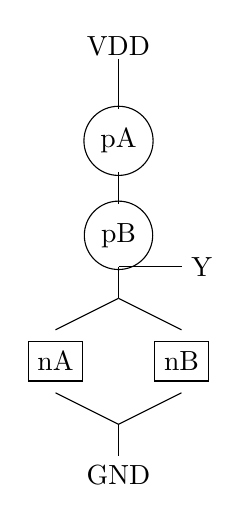
\begin{tikzpicture}[scale=0.8]
    % NOR
    \node at (0,4) {VDD};
    \draw (0,3.8) -- (0,3.5);
    % PUN Series
    \draw (0,3.5) -- (0,3);
    \node[draw,circle,minimum size=0.5cm] (pA) at (0,2.5) {pA};
    \draw (0,2) -- (0,1.5);
    \node[draw,circle,minimum size=0.5cm] (pB) at (0,1) {pB};
    % Output
    \draw (0,0.5) -- (1,0.5) node[right] {Y};
    % PDN Parallel
    \draw (0,0.5) -- (0,0);
    \draw (0,0) -- (-1,-0.5); \draw (0,0) -- (1,-0.5);
    \node[draw,rectangle,minimum size=0.5cm] (nA) at (-1,-1) {nA};
    \node[draw,rectangle,minimum size=0.5cm] (nB) at (1,-1) {nB};
    \draw (-1,-1.5) -- (0,-2); \draw (1,-1.5) -- (0,-2);
    \draw (0,-2) -- (0,-2.5) node[below] {GND};
\end{tikzpicture}
\\
\end{tabulary}
\end{center}
\end{solutionbox}

\begin{mnemonicbox}
\mnemonic{NAND: Parallel PMOS, Series NMOS. NOR: Series PMOS, Parallel NMOS.}
\end{mnemonicbox}

\questionmarks{4(c) OR}{7}{Implement Y=[PQ+R(S+T)]' Boolean equation using depletion load nMOS and CMOS.}

\begin{solutionbox}
\textbf{Function:} $Y = \overline{PQ + R(S+T)}$

\textbf{1. Depletion Load nMOS:}
PDN implements the function without inversion.
Structure: $S$ parallel $T$, in series with $R$. This block parallel with $P$ series $Q$.

\begin{center}
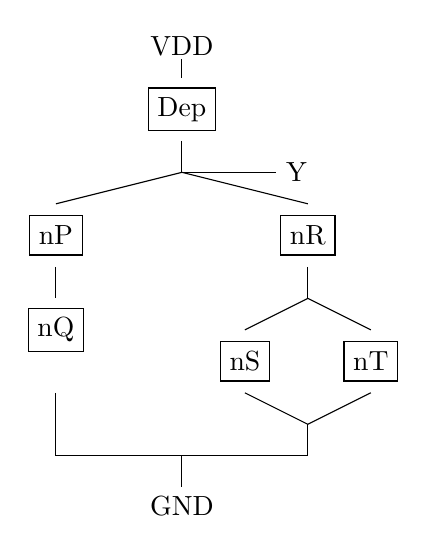
\begin{tikzpicture}[scale=0.8]
    \node at (0,5) {VDD};
    \draw (0,4.8) -- (0,4.5);
    % Depletion Load
    \node[draw,rectangle] (load) at (0,4) {Dep};
    \draw (0,3.5) -- (0,3);
    \draw (0,3) -- (1.5,3) node[right] {Y};
    
    % PDN
    % Branch 1: P-Q
    \draw (0,3) -- (-2,2.5);
    \node[draw,rectangle,minimum size=0.5cm] (nP) at (-2,2) {nP};
    \draw (-2,1.5) -- (-2,1);
    \node[draw,rectangle,minimum size=0.5cm] (nQ) at (-2,0.5) {nQ};
    
    % Branch 2: R(S+T)
    \draw (0,3) -- (2,2.5);
    \node[draw,rectangle,minimum size=0.5cm] (nR) at (2,2) {nR};
    \draw (2,1.5) -- (2,1);
    
    \draw (2,1) -- (1,0.5); \draw (2,1) -- (3,0.5);
    \node[draw,rectangle,minimum size=0.5cm] (nS) at (1,0) {nS};
    \node[draw,rectangle,minimum size=0.5cm] (nT) at (3,0) {nT};
    
    \draw (1,-0.5) -- (2,-1); \draw (3,-0.5) -- (2,-1);
    \draw (2,-1) -- (2,-1.5);
    
    \draw (-2,-0.5) -- (-2,-1.5);
    \draw (-2,-1.5) -- (2,-1.5) -- (0,-1.5);
    \draw (0,-1.5) -- (0,-2) node[below] {GND};
\end{tikzpicture}
\captionof{figure}{Depletion Load Implementation}
\end{center}

\textbf{2. CMOS Implementation:}
PDN is same as above. PUN is dual.
\textbf{Dual of PDN:}
Dual of $(S+T)$ is $S \cdot T$.
Dual of $R \cdot (S+T)$ is $R + (S \cdot T)$.
Dual of $P \cdot Q$ is $P + Q$.
Dual of $(P \cdot Q) + (R \cdot (S+T))$ is $(P+Q) \cdot (R + ST)$.
Structure: $(P || Q)$ in series with $(R || (S \text{ series } T))$.
\end{solutionbox}

\questionmarks{5(a)}{3}{Explain design styles used in Verilog.}

\begin{solutionbox}
\textbf{Verilog Design Styles:}

\begin{center}
\begin{tabulary}{\linewidth}{|L|L|L|}
\hline
\textbf{Style} & \textbf{Description} & \textbf{Example} \\ \hline
\textbf{Gate Level} & Structural modeling using primitive gates (and, or, not). & \code{and g1(y, a, b);} \\ \hline
\textbf{Data Flow} & Describes signal flow using continuous assignment. & \code{assign y = a \& b;} \\ \hline
\textbf{Behavioral} & Describes functionality using procedural blocks. & \code{always @(*) y = a \& b;} \\ \hline
\end{tabulary}
\end{center}

\textbf{Mnemonic}: \textit{Gate-Data-Behavior: Three ways to Model}
\end{solutionbox}

\questionmarks{5(b)}{4}{Write Verilog program for full adder using behavioral modeling.}

\begin{solutionbox}
\begin{lstlisting}[language=Verilog]
module full_adder_behavioral (
    input wire a, b, cin,
    output reg sum, cout
);

always @(*) begin
    case ({a, b, cin})
        3'b000: {cout, sum} = 2'b00;
        3'b001: {cout, sum} = 2'b01;
        3'b010: {cout, sum} = 2'b01;
        3'b011: {cout, sum} = 2'b10;
        3'b100: {cout, sum} = 2'b01;
        3'b101: {cout, sum} = 2'b10;
        3'b110: {cout, sum} = 2'b10;
        3'b111: {cout, sum} = 2'b11;
        default: {cout, sum} = 2'b00;
    endcase
end
endmodule
\end{lstlisting}
\end{solutionbox}

\questionmarks{5(c)}{7}{Describe the function of CASE statement. Write Verilog code of 3x8 decoder using CASE statement.}

\begin{solutionbox}
\textbf{CASE Statement:} Multi-way branching construct.
\textbf{Features:}
\begin{itemize}
    \item Compares expression with case items.
    \item Execute first matching item.
    \item \code{default} item covers unmatched cases.
\end{itemize}

\textbf{3x8 Decoder:}
\begin{lstlisting}[language=Verilog]
module decoder_3x8 (
    input wire [2:0] sel,
    input wire en,
    output reg [7:0] y
);
always @(*) begin
    if (en) begin
        case (sel)
            3'b000: y = 8'b00000001;
            3'b001: y = 8'b00000010;
            3'b010: y = 8'b00000100;
            3'b011: y = 8'b00001000;
            3'b100: y = 8'b00010000;
            3'b101: y = 8'b00100000;
            3'b110: y = 8'b01000000;
            3'b111: y = 8'b10000000;
            default: y = 8'b00000000;
        endcase
    end else y = 0;
end
endmodule
\end{lstlisting}
\end{solutionbox}

\questionmarks{5(a) OR}{3}{Write Verilog code to implement 2:1 multiplexer.}

\begin{solutionbox}
\begin{lstlisting}[language=Verilog]
// Behavioral
module mux21 (input a, b, s, output reg y);
    always @(*) begin
        if(s) y = b;
        else y = a;
    end
endmodule

// Data Flow
module mux21_df (input a, b, s, output y);
    assign y = s ? b : a;
endmodule
\end{lstlisting}
\end{solutionbox}

\questionmarks{5(b) OR}{4}{Write Verilog program for D flip-flop using behavioral modeling.}

\begin{solutionbox}
\begin{lstlisting}[language=Verilog]
module d_ff (
    input clk, rst, d,
    output reg q, qbar
);
always @(posedge clk or posedge rst) begin
    if (rst) begin
        q <= 0;
        qbar <= 1;
    end else begin
        q <= d;
        qbar <= ~d;
    end
end
endmodule
\end{lstlisting}
\end{solutionbox}

\questionmarks{5(c) OR}{7}{Explain testbench in brief. Write Verilog code to implement 4-bit down counter.}

\begin{solutionbox}
\textbf{Testbench:} A module used to verify design functionality by applying stimuli (inputs) and monitoring responses (outputs). It is non-synthesizable.

\textbf{4-bit Down Counter:}
\begin{lstlisting}[language=Verilog]
module down_counter (
    input clk, rst, en,
    output reg [3:0] count
);
always @(posedge clk or posedge rst) begin
    if (rst) count <= 4'b1111;
    else if (en) count <= count - 1;
end
endmodule
\end{lstlisting}

\textbf{Testbench Code:}
\begin{lstlisting}[language=Verilog]
module tb_counter;
    reg clk, rst, en;
    wire [3:0] count;
    
    down_counter dut (clk, rst, en, count);
    
    always #5 clk = ~clk;
    
    initial begin
        clk=0; rst=1; en=0;
        #10 rst=0; en=1;
        #200 $finish;
    end
    
    initial $monitor("T=%t C=%b", $time, count);
endmodule
\end{lstlisting}
\end{solutionbox}

\end{document}
